\newpage
You know what intercepts are.
They are where a graph of a function crosses the $x$- and $y$-axes.
So if you are given the graph of a function,
all you need to do to find the intercepts 
is look at the graph to see where the curve crosses the axes.
\begin{itemize}
    \item In some cases, you can see {\bfseries\itshape exactly} where it crosses
    if everything lines up nicely with the $x$-$y$ grid.
    \item But even if the curve doesn't cross the axes 
    an a point on the grid, you could still {\bfseries\itshape estimate} where 
    the crossing points are.
\end{itemize}

\begin{myConceptSteps}{To find the $x$- and $y$-intercepts given the graph of a relation\dots}
    \myStep{dots}{Draw a dot everywhere the curve crosses either axis.}
    \myStep{coordinates}{Find the ($x$,$y$) coordinates of those dots.}
    \myStep{$x$-intercepts}{
        The $x$-intercepts are the dots on the $x$-axis.
        You may write the intercept either as the point $(x,0)$ or just as the $x$ value.
    }
    \myStep{$y$-intercepts}{
        The $y$-intercepts are the dots on the $y$-axis.
        You may write the intercept either as the point $(0,y)$ or just as the $y$ value.
    }
\end{myConceptSteps}

\begin{myExample}{
    Find the $x$- and $y$-intercepts of this relation.
    \begin{center}
        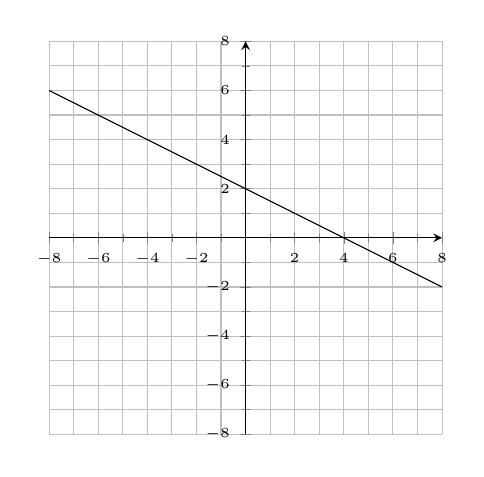
\begin{tikzpicture}
            \begin{axis}[
                width=3in,
                grid=both,
                axis x line = middle,axis y line = middle,
                axis equal image,
                xtick distance = 2, ytick distance = 2, 
                minor tick num = 1,
                xmin = -8, xmax=8,
                ymin = -8, ymax=8,
                tick label style = {font=\tiny},
                ]
                \addplot[no marks, samples=3, domain=-8:8, ] expression { -(1/2)*x + 2 }; 
            \end{axis}
        \end{tikzpicture}
    \end{center}
}
    \vspace{3in}
\end{myExample}


\begin{myExample}{
    Find the $x$- and $y$-intercepts of this relation.
    \begin{center}
        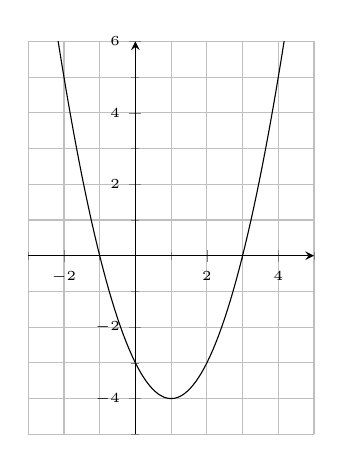
\begin{tikzpicture}
            \begin{axis}[
                width=3in,
                grid=both,
                axis x line = middle,axis y line = middle,
                axis equal image,
                xtick distance = 2, ytick distance = 2, 
                minor tick num = 1,
                xmin = -3, xmax=5,
                ymin = -5, ymax=6,
                tick label style = {font=\tiny},
                ]
                \addplot[no marks, samples=100, domain=-3:5, ] expression { (x-1)^2 - 4 };
            \end{axis}
        \end{tikzpicture}
    \end{center}
}
    \vspace{2in}
\end{myExample}